\section{System architecure}
\label{sec:system_architecture}

\subsection{\SeeDB\ overiew}
\label{subsec:overview}

Figure \ref{fig:sys-arch} shows the architecture of our system. Currently, 
\SeeDB\ is a wrapper around a database (PostgreSQL in this case). While
optimization opportunities are restricted by virtue of being outside the DBMS,
we believe that it allows quick iteration and permits \SeeDB\ to be used with
different backends. 

\begin{figure}[htb]
\centerline{
\hbox{\resizebox{9cm}{!}{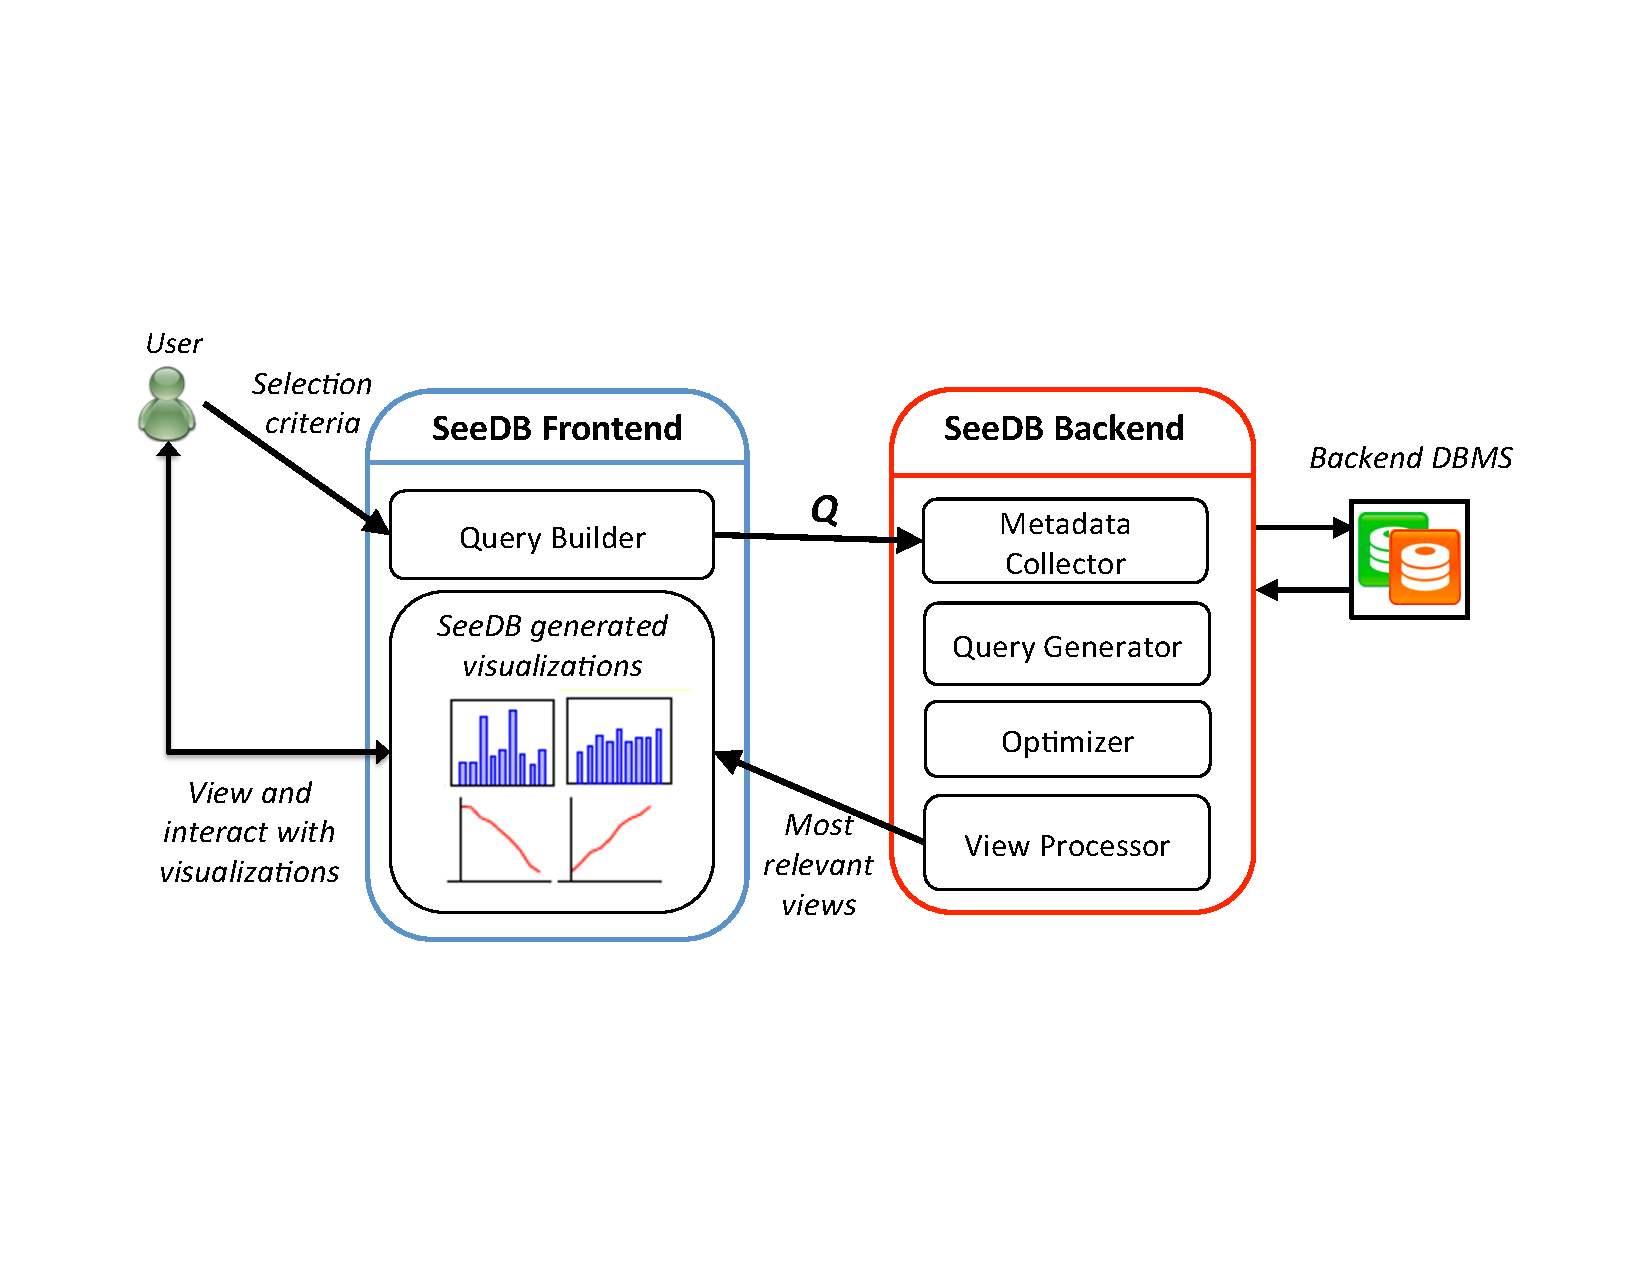
\includegraphics[trim=10mm 50mm 10mm 50mm,
clip=true]{Images/seedb-architecture.pdf}}}}
\caption{SeeDB Architecture}
\label{fig:sys-arch}
\end{figure} 

The \SeeDB\ frontend allows the user to pose queries via various means including
raw SQL, an easy-to-use query builder and a set of queries pre-written for
specific tasks (more in \ref{}). Once the user issues a query $Q$ to \SeeDB\,
the \SeeDB\ optimizer determines potential views possible for $Q$ and explores
options to optimize the computation of these views (Section \ref{}). These
options include traditional multi-query optimization techniques as well as
pruning heuristics. The View Query Generator module of \SeeDB\ then uses this
information to rewrite $Q$ as multiple queries where each query is either a view
or a precursor to multiple views. These queries are sent to the DBMS and the
results are processed by the Post-processor to generate data for individual
views and determine utility for each view. The views are then ranked using a
metric that depends both on the view utility and complexity of the view (we
prefer views with high utility and low complexity). The top-k views with highest
utility are then picked and shipped to the frontend. The post-processor also
determines the best way to package view information to allow quick future
interaction at the frontend. The SeeDB frontend uses view information sent by
the SeeDB engine to pick appropriate visualizations and show the top views along
with appropriate metadata. The user can then examine these views and perform
further processing (Section \ref{}).

\subsection{Basic Framework}
\label{basic_framework}

Given a user query $Q$, the basic version of \SeeDB\ computes all possible view
queries by adding a single aggregate and a single or multiple attribute group-by
operator to $Q$. Each of these view queries is executed independently at the
backend along with an equivalent aggregate+group-by query on the complete
underlying dataset. These two query results produce a ``distribution'' for the
attribute that has been aggregated (Section \ref{}). These two distributions are
compared using the chosen distance metric (Section \ref{}) and the top k views
with the largest distance are chosen. These views are sent to the
frontend where they are visualized and presented to the user (Section
\ref{user_interface}).
% {\bf Utility Metric}:
% 
% One of the key challenges behind \SeeDB\ 
% is formalizing the utility function $U(R)$ for a discriminating view $R$. 
% There are many choices for $U$ and we expect \SeeDB\ 
% to recommend views that score high on several metrics. 
% As discussed previously, the proposed metric tries to capture the idea of
% ``deviation'' between distributions, i.e., a view has high utility if its
% contents show a trend that deviates from the corresponding trend in the original
% database.
% 
% We first define some notation. For any discriminating view $R_i$ 
% in the class defined above, we note that $R_i(D)$ and $R_i(Q(D))$ 
% are both two column tables. 
% A two-column table can be represented using a weight vector.
% We let the weight vector $W_{a, f(m)}$ represent the 
% result of $R_i(D) = \gamma_{a, f(m)}(D)$, i.e., 
% distribution of the aggregate function $f$ on the measure quantity $m$ 
% across various values of the attribute $a$. 
% 
% The utility $U$ of a discriminating view $\gamma_{a, f(m)}$ is defined to be the
% distance between $W_{a, f(m)}^Q$, and $W_{a, f(m)}$:
% $U(\gamma_{a, f(m)}) = S(W_{a, f(m)}^Q, $ $W_{a, f(m)})$ where $S$ is a distance
% metric. The higher $S$ is, the more useful a discriminating view is.
% Common distance metrics used in visualization literature include K-L
% divergence~\cite{wikipedia-KL}, Jenson-Shannon
% distance~\cite{wikipedia-JS,entropy-vis}, and earth mover
% distance~\cite{wikipedia-prob-dist}.
% Wang~\cite{entropy-vis} provides a good overview of the metrics used in
% scientific visualizations, while \cite{wikipedia-prob-dist} provides a summary
% of probability-based distance metrics.
% As discussed earlier, we do not prescribe any specific distance metrics,
% instead, we plan to support a whole range of distance metrics, which can be
% overridden by the data analyst.

\subsection{Optimizations}
\label{optimizations}

Since \SeeDB\ executes many similar queries, we clearly can do better than
the basic algorithm presented above, and \SeeDB\ implements various such
optimizations. Strategies include:

\begin{enumerate}
  \item {\it Rewrite view query}: Since similar group-by and aggregate queries
  are executed on the results of user query $Q$ and the underlying dataset, we
  can combine these queries into one query. As shown in Figure \ref{}.a this
  achieves a speed-up of Y\%.
  \item {\it Single Group-by Multiple Aggregates}: A large number of view
  queries have the same group-by clause but aggregates on different attributes.
  A straightforward optimization combines all view queries with the same
  group-by clause into a single view query. This rewriting provides a speed up
  linear in the number of aggregate attributes. (Figure \ref{}. b).
  \item {\it Multiple Aggregate Computation}: Similar to data cubes (\cite{}),
  \SeeDB\ seeks to compute group-bys for a large set of attributes. One
  optimization is to combine queries with different group-by attributes into a
  single query with multiple group-bys. For instance, consider view queries
  $V(Q, A_1, G_1)$, $V(Q, A_1, G_2)$ \ldots $V(Q, A_1, G_n)$. Instead of
  executing them individually, we can rewrite them into a single view query
  $V(Q, A_1, (G_1, G_2\ldots G_n))$. While this strategy reduces query
  execution time, \SeeDB\ must spend more time combining the results and
  obtaining separate aggregates for individual $G_i$'s. This is reminiscent of
  data cube algorithms. As shown in Figure \ref{}.c the speed up depends closely
  on the number of distinct values for each of the group-by attributes and the
  memory constraints of the DBMS. A variation of this approach also implemented
  on \SeeDB\ is to send the results of the multiple group-by query to the front
  end and ask the \SeeDB\ frontend to compute utility and select views. The
  advantage of this approach is that it allows for more efficient interactive
  exploration of the views.
  \item {\it Sampling}: The final optimization we study for the purpose of this
  demo is sampling. Instead of running queries on the entire dataset, we
  run queries on subsets of the data at the expense of reduced accuracy.
  Figure \ref{}.d shows the effects of this optimization. As expected, the
  sampling technique and size of the sample can affect the accuracy of the
  generated views. As a result, the user can specify whether inaccuracies are
  acceptable and therefore, whether \SeeDB\ can use sampling.
  
  Although other optimizations are possible, particularly related to
  pre-computing aggregate results, we discuss them in the full paper currently
  in preparation.
\end{enumerate}

\subsection{User Interface}
\label{user_interface}

%\begin{figure}[htb]
%\centerline{
%\hbox{\resizebox{9cm}{!}{\includegraphics[trim=10mm 50mm 10mm 50mm,
%clip=true]{Images/seedb-frontend.pdf}}}}
%\caption{SeeDB Frontend}
%\label{fig:frontend}
%\end{figure} 
<<figure goes here after I get it from Angela/Sashko>>

The \SeeDB\ frontend serves two purposes - to input a query, and to visualize
and analyze the resulting views. We provide the user with three options for
specifying an input query: (a) as raw SQL, (b) through a query builder that can
allow users unfamiliar with SQL to formulate queries through an easy-to-use
form-based interface, (c) through pre-defined query templates, e.g., queries
that select outliers in a particular column. These templates are particularly
useful since users are interested in anomalous data points.

Once a user submits a query to \SeeDB\, the \SeeDB\ engine evaluates various
views and sends the most promising ones to the frontend. The frontend then
determines the best ways to visualize these views (e.g. depending on data types
being represented, number of distinct values etc.) and displays the
visualizations. The user can then examine these diverse views at a glance,
explore specific views in detail and view metadata for each view (e.g. size of
result, sample data, value with maximum change, statistics etc.). The user can
also slice-and-dice views further by selecting particular values of grouping
attributes to explore. The user does this simply by selecting the relevant
attribute values in the view. This automatically modifies the selection query
and displays views for the subset of data selected. The user can of course
revert back to the original views and continue exploring the data.
